\documentclass[10pt]{article}
\usepackage[margin=0.9in]{geometry}
\usepackage{amsmath,amssymb}
\usepackage{graphicx}
\usepackage{booktabs}
\usepackage[hidelinks]{hyperref}
\graphicspath{{../figures/}}
\setlength{\parindent}{0pt}
\setlength{\parskip}{4pt}

\title{\vspace{-2.2cm}Improved PINNs for option pricing: an implementation of Bai, Chaolu \& Bilige (2022)}
\author{Sondre Rogde, CEE292 Project 1, November 2026}
\date{}
\usepackage{float}
\setlength{\intextsep}{6pt}
\setlength{\abovecaptionskip}{4pt}

\begin{document}
\maketitle
\vspace{-2em}

\section{Introduction}

Bai, Chaolu and Bilige \cite{bai2022} apply physics-informed neural networks (PINNs, \cite{raissi2019})
to two option-pricing PDEs, the nonlinear Ivancevic equation and the Black--Scholes equation, and
propose an ``improved PINN'' (IPINN) that adds the neuron-wise locally adaptive activation functions
with slope recovery of Jagtap et al.\ \cite{jagtap2020}. They claim that their proposed IPINN converges faster 
and with slightly better accuracy than the plain PINN on a financial rogue wave, a soliton, and a European call.

This project implements both the PINN and the IPINN in PyTorch and runs the same three experiments of the paper
with 5 random seeds each. The main result is negative: the IPINN loss as written in the paper is
unbounded below in the activation slopes, and the L-BFGS phase of training exploits this, saturating
the network. With the slope-recovery term removed, the adaptive activations train fine but are not
better than the plain PINN on these problems. Code and results: \url{https://github.com/REPO-LINK}.

\section{Methods}

\subsection{PINN and IPINN}

A fully connected network $\hat u_\theta(S,t)$ with 8 hidden tanh layers approximates the PDE solution.
It is trained on the usual PINN loss we have seen in class:
\begin{equation}
  \mathcal{L}_{\text{total}} = \mathcal{L}_{\text{data}} + \mathcal{L}_{\text{physics}}, \quad
  \mathcal{L}_{\text{data}} = \frac{1}{N_{\text{data}}}\sum_{i} \big|\hat u_\theta(S_i,t_i) - u_i\big|^2, \quad
  \mathcal{L}_{\text{physics}} = \frac{1}{N_{\text{colloc}}}\sum_{j} \big|\mathcal{R}_\theta(S_j,t_j)\big|^2,
\end{equation}
where the data points lie on the initial and boundary lines, the collocation points are Latin-hypercube
samples of the domain, and the residual $\mathcal{R}_\theta$ is the PDE evaluated on $\hat u_\theta$ with
automatic differentiation. Training is Adam followed by L-BFGS.

The IPINN keeps this loss but replaces every hidden activation by $\tanh(n\,a\,z)$ with one trainable
slope $a$ per neuron ($n=10$, $a=0.1$ at initialisation, i.e.\ a plain tanh network at the start) and adds
the slope-recovery term of \cite{jagtap2020},
\begin{equation}
  \mathcal{L}_{\text{IPINN}} = \mathcal{L}_{\text{total}} + S(a), \qquad
  S(a) = \Big[\text{mean}_{\text{layers}}\, \exp\big(\text{mean}_{\text{neurons}}\, a\big)\Big]^{-1},
  \label{eq:sr}
\end{equation}
which is meant to push the slopes up and speed up training. Because this term turned out to break
training (Section~\ref{sec:results}), a third variant with adaptive slopes but without $S(a)$ is also
run, labelled ``IPINN w/o slope recovery''.

\subsection{Problems}

The Ivancevic model is the nonlinear Schr\"odinger equation
$i\psi_t + \tfrac{\sigma}{2}\psi_{SS} + \beta|\psi|^2\psi = 0$ for a complex option-price wave function
$\psi(S,t)$. The network outputs the real and imaginary parts and the residual has two components.
As in the paper we solve for the financial rogue wave of Yan \cite{yan2010}
($\sigma=\beta=1$ on $S\in[-2,2]$, $t\in[-1.5,1.5]$) and a bright soliton
($\sigma=\beta=2$, $\psi = 2\,\mathrm{sech}(2S+8t)\,e^{i(1-2S)}$ on $S\in[-5,5]$, $t\in[-0.5,0.5]$).
The Black--Scholes equation is given by, $V_\tau = \tfrac12\sigma^2 S^2 V_{SS} + rSV_S - rV$, with initial condition $V(S,0)=\max(S-K,0)$. We have
$K=10$, $r=0.1$, $\sigma=0.05$ on $S\in[0,20]$, $\tau\in[0,1]$. All three have closed-form solutions,
which are used for the training data and the test errors.

\subsection{Training and evaluation}

Network sizes (8 hidden layers of 40 units for Ivancevic, 50 for Black--Scholes), the number of data
points ($N_{\text{data}} = 100$ and $200$) and the collocation points of the Ivancevic problems follow the
paper. Table~\ref{tab:setup} lists where we deviate. The reductions were made so that all 45 runs fit in
about two hours on a laptop (Apple M2); . I also did a check with 5000 Adam steps on one see which did not
change the results significantly. Errors are the relative $L^2$ error and the maximum absolute error on a
dense grid, reported as mean $\pm$ std over the 5 seeds. The seed changes both the sampled points and
the initialization.

\begin{table}[H]
  \centering
  \caption{Our setup versus the paper's.}
  \label{tab:setup}
  \small
  \begin{tabular}{lll}
    \toprule
     & this project & paper \\
    \midrule
    Adam steps & 2000 (lr $10^{-3}$) & 10\,000 \\
    L-BFGS iterations & up to 5000 (strong Wolfe, stops on tolerance) & 15\,000 \\
    $N_{\text{colloc}}$, Black--Scholes call & 2000 & 10\,000 \\
    Black--Scholes training data & closed-form solution & finite-difference solver \\
    Precision & single & not stated \\
    Runs per experiment & 5 seeds, mean $\pm$ std & 1 \\
    \bottomrule
  \end{tabular}
\end{table}

\section{Results}
\label{sec:results}

\begin{table}[H]
  \centering
  \caption{Test errors, mean $\pm$ std over 5 seeds.}
  \label{tab:results}
  \small
  \begin{tabular}{llcc}
\toprule
problem & method & relative $L^2$ error & max.\ abs.\ error \\
\midrule
Black-Scholes call & PINN & $(4.69 \pm 1.42) \times 10^{-4}$ & $(6.19 \pm 1.32) \times 10^{-2}$ \\
 & IPINN w/o slope recovery & $(4.26 \pm 0.51) \times 10^{-4}$ & $(6.21 \pm 0.67) \times 10^{-2}$ \\
 & IPINN & $(5.19 \pm 1.49) \times 10^{-3}$ & $(4.98 \pm 4.41) \times 10^{-1}$ \\
Ivancevic soliton & PINN & $(4.30 \pm 0.55) \times 10^{-2}$ & $(1.42 \pm 0.20) \times 10^{-1}$ \\
 & IPINN w/o slope recovery & $(6.87 \pm 3.14) \times 10^{-2}$ & $(2.36 \pm 1.05) \times 10^{-1}$ \\
 & IPINN & $(1.08 \pm 0.03) \times 10^{0}$ & $(2.60 \pm 0.05) \times 10^{0}$ \\
Ivancevic rogue wave & PINN & $(2.72 \pm 1.28) \times 10^{-2}$ & $(9.40 \pm 3.99) \times 10^{-2}$ \\
 & IPINN w/o slope recovery & $(4.42 \pm 1.01) \times 10^{-2}$ & $(1.49 \pm 0.33) \times 10^{-1}$ \\
 & IPINN & $(9.23 \pm 0.14) \times 10^{-1}$ & $(3.74 \pm 0.01) \times 10^{0}$ \\
\bottomrule
\end{tabular}

\end{table}

Our results agree with the paper on the plain PINN and disagree on the IPINN. For the standard PINN, our rogue-wave error is below the $7.3\times10^{-2}$ the original paper reports.
The Black--Scholes error is an order of magnitude below their $8.2\times10^{-3}$. This is most likely because our training
data is exact, while they used a finite difference solution. The soliton error is an order of magnitude above
their $2.6\times10^{-3}$, which might be due to the smaller training budget. 

The IPINN as written, however,
diverges on both Ivancevic problems and is ten times worse than PINN on Black--Scholes, on every seed.
Figure~\ref{fig:loss} shows that $S(a)$ in Eq.~\eqref{eq:sr} has no lower bound except $0$ at
$a\to\infty$ and is still about $0.8$ after the Adam phase, far above the PDE loss, so L-BFGS lowers the
total loss by inflating the slopes instead of fitting the PDE. The mean effective slope $na$ grows from $1$
to $5$--$19$, single neurons reach $56$, the tanh units saturate and the network collapses to a nearly
constant function. Without $S(a)$ the slopes stay near $1$ and the adaptive network trains like the plain
PINN, slightly better on Black--Scholes and somewhat worse on the Ivancevic problems.

\begin{figure}[H]
  \centering
  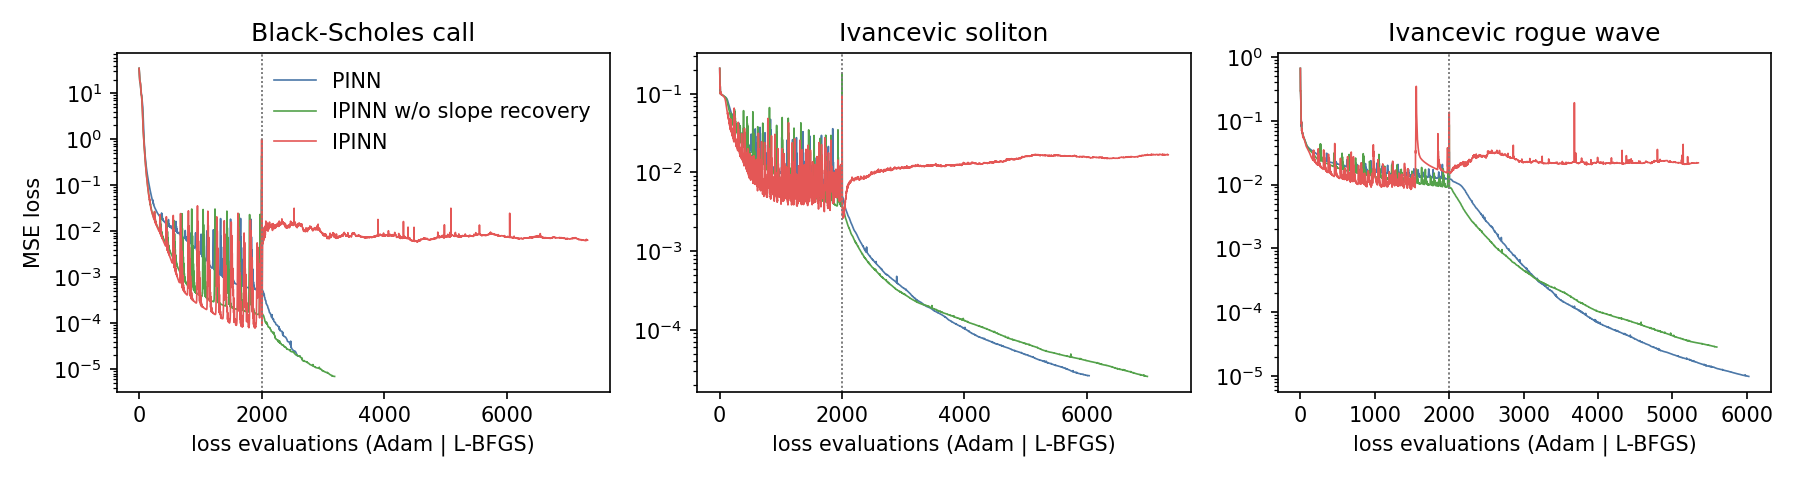
\includegraphics[width=0.85\textwidth]{loss.png}
  \caption{PDE-and-data part of the loss (without $S(a)$) during training for seed 0. The dotted line
  marks the switch from Adam to L-BFGS. For the paper's IPINN the loss rises during L-BFGS while the
  optimizer lowers $S(a)$ by inflating the slopes.}
  \label{fig:loss}
\end{figure}

\section{Conclusion}

The plain PINN from the paper was straightforward to reproduce and works on all three problems with a
much smaller training budget than the paper used. The improved version did not work for us. It seems like the extra
loss term rewards ever larger activation slopes. The paper does not
report the learned slopes or any bound on the term, so it is hard to tell how its runs avoided this. It might be avoided
by weighing the slope-recovery term differently.
More plots and results can be found in the GitHub repo.

\footnotesize
\begin{thebibliography}{9}
\bibitem{bai2022} Y. Bai, T. Chaolu, S. Bilige. The application of improved physics-informed neural
  network (IPINN) method in finance. \emph{Nonlinear Dyn.} 107, 3655--3667 (2022).
\bibitem{raissi2019} M. Raissi, P. Perdikaris, G. E. Karniadakis. Physics-informed neural networks.
  \emph{J. Comput. Phys.} 378, 686--707 (2019).
\bibitem{jagtap2020} A. D. Jagtap, K. Kawaguchi, G. E. Karniadakis. Locally adaptive activation
  functions with slope recovery for deep and physics-informed neural networks.
  \emph{Proc. R. Soc. A} 476, 20200334 (2020).
\bibitem{yan2010} Z. Yan. Financial rogue waves. \emph{Commun. Theor. Phys.} 54, 947--949 (2010).
\end{thebibliography}

\end{document}
